\documentclass[../../../include/open-logic-section]{subfiles}

\begin{document}

\olfileid{sth}{ordinals}{idea}
\olsection{क्रमसूचक संख्येची सर्वसाधारण कल्पना}

नैसर्गिक संख्यांचा नेहमीचा क्रम पाहा:
\begin{center}
	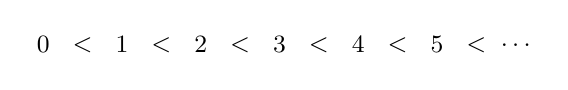
\begin{tikzpicture}
	\foreach \x/\xtext in {0, 1, 2, 3, 4, 5}
	{
		\node (\x a) at (\x, 1) {\small{$\x$}};
		\node (\x a) at (\x.5, 1) {\small{$<$}};
	}
	\node (ldots) at (6, 1) {\small{$\ldots$}};
	\end{tikzpicture}
\end{center}
याला तांत्रिक भाषेत $\omega$-अनुक्रम म्हणतात. संचांच्या पदानुक्रमातील सुरुवातीचे टप्पे बांधताना हीच सर्वसाधारण क्रमरचना दिसते. आता या अनुक्रमातील $0$ बाकी सर्व संख्यांच्या शेवटी नेऊ:
\begin{center}
	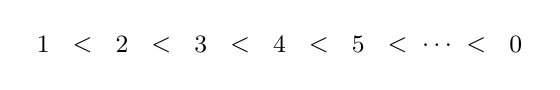
\begin{tikzpicture}
	\foreach \x/\xtext in {1, 2, 3, 4, 5}
	{
		\node (\x a) at (\x, 1) {\small{$\x$}};
		\node (\x a) at (\x.5, 1) {\small{$<$}};
	}
	\node (ldots) at (6, 1) {\small{$\ldots$}};
	\node (bea) at (6.5, 1) {\small{$<$}};
	\node (noa) at (7, 1) {\small{$0$}};
	\end{tikzpicture}
\end{center}
येथे घटक तेच आहेत; पण त्यांचा क्रम मुळात वेगळा आहे. पहिल्या क्रमाला शेवटचा घटक नव्हता; नव्या क्रमाला आहे. या नव्या क्रमात घटकांचा $\omega$-अनुक्रम ($1, 2, 3, 4, 5, \ldots$) आहे आणि त्यानंतर आणखी एक घटक येतो. म्हणून तो $\omega+1$-अनुक्रम आहे.

हेच घटक वापरून आणखी वेगवेगळ्या प्रकारचे क्रम बनवता येतात. उदाहरणार्थ, सर्व सम संख्या त्यांच्या नेहमीच्या क्रमात आणि त्यानंतर सर्व विषम संख्या त्यांच्या नेहमीच्या क्रमात घ्या:
\begin{center}
	\begin{tikzpicture}
	\node(a1) at (1,1) {\small{$0$}};
	\node(a2) at (1.5,1) {\small{$<$}};
	\node(a3) at (2,1) {\small{$2$}};
	\node(a4) at (2.5,1) {\small{$<$}};
	\node(a5) at (3,1) {\small{$4$}};
	\node(a6) at (3.5,1) {\small{$<$}};
	\node(dots) at (4,1) {\small{$\ldots$}};
	\node(aaoe) at (4.5,1) {\small{$<$}};
	\node(b1) at (5,1) {\small{$1$}};
	\node(b2) at (5.5,1) {\small{$<$}};
	\node(b3) at (6,1) {\small{$3$}};
	\node(b4) at (6.5,1) {\small{$<$}};
	\node(b5) at (7,1) {\small{$\ldots$}};
	\end{tikzpicture}
\end{center}
हा एका $\omega$-अनुक्रमानंतर दुसरा $\omega$-अनुक्रम आहे; म्हणजे $\omega+\omega$-अनुक्रम.

असे पुढेही करता येईल. पण \emph{क्रमरचनांविषयी} ही चर्चा समजून घेण्यासाठी आपल्याला एक सर्वसाधारण पद्धत हवी आहे.

\end{document}
